\documentclass[draft, twocolumn]{article}
\usepackage[unicode,draft=false,hidelinks]{hyperref}
\usepackage{cite}
\usepackage{catchfilebetweentags}
\usepackage{amssymb}
\usepackage{turnstile}
\usepackage{bbm}
\usepackage[greek, english]{babel}
\usepackage{MnSymbol}
\usepackage{stmaryrd}
\usepackage{csquotes}
\newcommand\doubleplus{+\kern-1.3ex+\kern0.8ex}
\newcommand\mdoubleplus{\ensuremath{\mathbin{+\mkern-8mu+}}}
\makeatletter
\newcommand\incircbin
{%
  \mathpalette\@incircbin
}
\newcommand\@incircbin[2]
{%
  \mathbin%
  {%
    \ooalign{\hidewidth$#1#2$\hidewidth\crcr$#1\bigcirc$}%
  }%
}
\newcommand{\oeq}{\ensuremath{\incircbin{=}}}
\makeatother
\makeatletter
\newcommand\insquarebin
{%
  \mathpalette\@insquarebin
}
\newcommand\@insquarebin[2]
{%
  \mathbin%
  {%
    \ooalign{\hidewidth$#1#2$\hidewidth\crcr$#1\bigbox$}%
  }%
}
\newcommand{\sqtri}{\ensuremath{\insquarebin{\triangle}}}
\makeatother
\usepackage{ucs}
\DeclareUnicodeCharacter{8759}{\ensuremath{\squaredots}}
\DeclareUnicodeCharacter{951}{\textgreek{\texteta}}
\DeclareUnicodeCharacter{737}{\ensuremath{^\text{l}}}
\DeclareUnicodeCharacter{691}{\ensuremath{^\text{r}}}
\DeclareUnicodeCharacter{7523}{\ensuremath{_\text{r}}}
\DeclareUnicodeCharacter{8718}{\ensuremath{\blacksquare}}
\DeclareUnicodeCharacter{957}{\textgreek{\textnu}}
\DeclareUnicodeCharacter{961}{\textgreek{\textrho}}
\DeclareUnicodeCharacter{929}{\textgreek{\textRho}}
\DeclareUnicodeCharacter{954}{\textgreek{\textkappa}}
\DeclareUnicodeCharacter{10214}{\ensuremath{\lsem}}
\DeclareUnicodeCharacter{10215}{\ensuremath{\rsem}}
\DeclareUnicodeCharacter{8857}{\mdoubleplus}
\DeclareUnicodeCharacter{8860}{\oeq}
\DeclareUnicodeCharacter{9043}{\ensuremath{\sqtri}}
\DeclareUnicodeCharacter{928}{\textgreek{\textPi}}
\DeclareUnicodeCharacter{922}{\textgreek{\textKappa}}
\DeclareUnicodeCharacter{931}{\textgreek{\textSigma}}
\DeclareUnicodeCharacter{916}{\textgreek{\textDelta}}
\DeclareUnicodeCharacter{8779}{\ensuremath{\backtriplesim}}
\DeclareUnicodeCharacter{8799}{\ensuremath{\stackrel{?}{=}}}
\DeclareUnicodeCharacter{10181}{\ensuremath{\lbag}}
\DeclareUnicodeCharacter{10182}{\ensuremath{\rbag}}
\DeclareUnicodeCharacter{8760}{\ensuremath{-}}
\usepackage[utf8x]{inputenc}
\usepackage[T1]{fontenc}
\usepackage{autofe}
\usepackage[references]{agda}
\usepackage{bbding}
\setlength{\marginparwidth}{2cm}
\usepackage[obeyDraft]{todonotes}
\usepackage{lineno}
\setlength\linenumbersep{-0.5cm}
\usepackage{amsthm}
\theoremstyle{definition}
\newtheorem{definition}{Definition}[section]
\theoremstyle{definition}
\newtheorem{principle}{Principle}[section]
\usepackage{subcaption}
\usepackage{graphicx}
\usepackage{tikz}
\usetikzlibrary{decorations.pathmorphing}
\usetikzlibrary{snakes}
\usetikzlibrary{arrows}
\usetikzlibrary{cd}
\usepackage{forest}
\author{Donnacha Oisín Kidney}
\title{Automatically And Efficiently Illustrating Polynomial Equalities in Agda}
\begin{document}
\maketitle
\begin{abstract}
  We present a new library which automates the construction of equivalence
  proofs between polynomials over commutative rings and semirings in the
  programming language Agda\cite{norell_dependently_2008}. We use Agda's
  reflection machinery to provide a simple interface to the solver, and
  demonstrate a novel use of the constructed relations.
\end{abstract}
\tableofcontents
\section{Introduction}
Proof assistants and computer algebra systems (CASs) share many of the same
goals: fundamentally, they aim to leverage computer automation to assist a
mathematician, in much the same way that a word processor might help a writer.
One promising avenue for the development of proof assistants uses dependently
typed programming languages, like Agda\cite{norell_dependently_2008} and
Coq\cite{the_coq_development_team_2018_1219885}, to automate \emph{verification}
of proofs. Based on constructivist mathematics, these languages allow the
programmer to write proofs as \emph{programs}, which are then verified by the
compiler.

Before they achieve the same widespread usefulness of other CASs, however, these
languages have a significant hurdle to overcome: tedium. Truly formal proofs of
even basic mathematical identities are notoriously verbose (Russell and
Whitehead required 378 pages of preamble before proving \(1+1=2\)
\cite{whitehead_principia_1910}). While Coq and Agda have vastly improved the
situation, they still often suffer from a degree of explicitness that makes even
elementary identities daunting: used in the naïve way, equivalence proofs
require the programmer to specify every individual step (``here we rely on the
commutativity of \(+\), followed by the associativity of \(\times\) on its
right-hand-side'', and so on).

However, the real promise of dependently-typed languages lies not in the fact
that their programs are proofs, but rather the reverse: \emph{their proofs are
  programs}. There is nothing stopping us from implementing standard CAS
algorithms \emph{in the languages themselves}, and using those algorithms to
automate the construction of proofs. In doing so we go a step beyond the
capabilities of most CASs, proving correctness as well as automating it.
\subsection{Related Work} 
In dependently-typed programming languages, the state-of-the-art solver for
polynomial equalities (over commutative rings) was originally presented
in\cite{gregoire_proving_2005}, and is used in Coq's \verb+ring+ solver. This
work improved on the already existing solver\cite{Coq:manual} in both efficiency
and flexibility. In both the old and improved solvers, a reflexive technique
(section~\ref{reflexive}) is used to automate the construction of the proof
obligation (as described in\cite{boutin_using_1997}).

Agda\cite{norell_dependently_2008} is a dependently-typed programming language
based on Martin-Löf's Intuitionistic Type
Theory\cite{martin-lof_intuitionistic_1980}. Its standard
library\cite{danielsson_agda_2018} currently contains a ring solver which is
similar in flexibility to Coq's \verb+ring+, but doesn't support the
reflection-based interface, and is less efficient due to its use of a dense
(rather than sparse) internal data structure.

In\cite{geuvers_automatically_2017}, an implementation of an automated solver
for the dependently-typed language Idris\cite{brady_idris_2013} is described.
The solver is implemented with a ``correct-by-construction'' approach, in
contrast to\cite{gregoire_proving_2005}. The solver is defined over
\emph{non}commutative rings, meaning that it is more general (can work with more
types) but less powerful (meaning it can prove fewer identities). It provides a
reflection-based interface, but internally uses a dense representation.

Reflection and metaprogramming are relatively recent additions to Agda, but form
an important part of the interfaces to automated proof procedures. Reflection in
dependent types in general is explored in\cite{christiansen_practical_2015}, and
specific to Agda in\cite{van_der_walt_reflection_2012}.

Formalization of mathematics in general is an ongoing project.
\cite{wiedijk_formalizing_2018} tracks how much of ``The 100 Greatest Theorems''
\cite{kahl_hundred_2004} have so far been formalized (at time of writing, the
number stands at 93). DoCon\cite{meshveliani_docon-provable_2018} is a notable
Agda library in this regard: it contains many tools for basic maths, and
implementations of several CAS algorithms. Its implementation is described
in\cite{meshveliani_dependent_2013}. \cite{cheng_functional_2018} describes the
manipulation of polynomials in both Haskell and Agda.

Finally, the study of \emph{pedagogical} CASs which provide step-by-step
solutions is explored in\cite{lioubartsev_constructing_2016}. One of the most
well-known such system is Wolfram
Alpha\cite{wolfram_research_inc._wolframalpha_2019}, which has step-by-step
solutions\cite{the_development_team_step-by-step_2009}.
\subsection{Contributions}
\begin{description}
  \item[An New, Efficient Ring Solver]
    We provide an implementation of a polynomial solver in the programming
    language Agda. It improves on the old solver by using a sparse internal
    representation as in \cite{gregoire_proving_2005}. We also verify the
    optimizations.
  \item[Techniques For Efficient Verification] We demonstrate several techniques
    to thread verification and proof logic through algorithms \emph{without}
    changing complexity class. These techniques are of general use in functional
    languages with type systems powerful enough to express invariants.

    We also demonstrate a use of the Algebra of Programming approach in
    Agda\cite{mu_algebra_2009}.
  \item[A Simple Reflection-Based Interface] We use Agda's reflection machinery
    to provide the following interface to the solver:
    \ExecuteMetaData[Introduction.tex]{lemma}
    It imposes minimal overhead on the user: only the \(\AgdaDatatype{Ring}\)
    implementation is required, with no need for user implementations of
    quoting. Despite this, it is generic over any type which implements ring. To
    our knowledge, such an interface does not exist in Agda.
  \item[A Pedagogical Computer-Algebra System] We show how our solver can
    generate ``step-by-step'' solutions for the equalities, with no modification
    of the original code.
\end{description}
All of these contributions, while developed together, are entirely modular. For
instance, both the reflection interface \emph{and} the pedagogical solutions
work with the old version of the ring solver.
\section{The Reflexive Technique} \label{reflexive}
Before describing the specifics of a given solver algorithm, it's important to
understand how that algorithm can be applied in a dependently-typed language.
How do we go from goal to proof? How do we describe the goal? How do we
instantiate the proof?

We use a reflexive technique\cite{boutin_using_1997}. Rather than explaining it
\emph{and} the algorithm for solving rings all at once, we're first going to
illustrate the technique with a simpler algebra: \emph{monoids}.
\begin{definition}[Monoids]
  A monoid is a set equipped with a binary operation, \(\bullet\), and a
  distinguished element \(\epsilon\), such that the following equations hold:
  \begin{align}
    x \bullet (y \bullet z) &= (x \bullet y) \bullet z \tag{Associativity} \\
    x \bullet \epsilon      &= x \tag{Left Identity} \\
    \epsilon \bullet x      &= x \tag{Right Identity}
  \end{align}
  Addition and multiplication (with 0 and 1 being the respective identity
  elements) are perhaps the most obvious instances of the algebra. In computer
  science, monoids have proved a useful abstraction for formalizing concurrency
  (in a sense, an associative operator is one which can be evaluated in any
  order).
\end{definition}
In this section, we'll write a simple monoid solver. In the next, we will swap
out monoids for commutative rings to get the full solver.
\subsection{A ``Trivial'' Identity}
\begin{figure}[h]
  \ExecuteMetaData[Monoids.tex]{mon-ident}
  \caption{A Simple Identity Of Monoids}
  \label{mon-ident}
\end{figure}

As a running example for this section, we will use the identity in
figure~\ref{mon-ident}. To a human, the fact that the identity holds may well be
obvious: \(\AgdaField{∙}\) is associative, so we can scrub out all the
parentheses, and \(\AgdaField{ε}\) is the identity element, so scrub it out too.
After that, both sides are equal, so voilà! 

Unfortunately, our compiler isn't nearly that clever. As alluded to before, we
need to painstakingly specify every intermediate step, justifying every move:

\begin{samepage}
  \begin{linenumbers}
    \ExecuteMetaData[Monoids.tex]{mon-proof}
  \end{linenumbers}
\end{samepage}

The syntax is designed to mimic that of a handwritten proof: line 3 is the
expression on the left-hand side of \(\AgdaField{≈}\) in figure~\ref{mon-ident},
and line 9 the right-hand-side. In between, the expression is repeatedly
rewritten into equivalent forms, with justification provided inside the angle
brackets. For instance, to translate the expression from the form on line 3 to
that on line 5, the associative property of \(\AgdaField{∙}\) is used on line 4.

One trick worth pointing out is on line 6: the \(\AgdaFunction{∙-cong}\) lifts
two equalities to either side of a \(\AgdaField{∙}\). In other words, given
proofs of the following:
\begin{align*}
x_1 \;&\AgdaField{≈} \; x_2 \\
y_1 \;&\AgdaField{≈} \; y_2
\end{align*}
it will prove:
\[x_1 \; \AgdaField{∙} \; y_1 \; \AgdaField{≈} \; x_2 \; \AgdaField{∙} \; y_2\]


This function needs to be explicitly provided by the user, as we only require
\(\AgdaField{≈}\) to be an equivalence relation (rather than, say, requiring
that it be true propositional equality). Section~\ref{equivalence} explains why
this is useful.
\subsection{ASTs for the Language of Monoids}
The first hurdle for automatically constructing proofs comes from the fact that
the identity in figure~\ref{mon-ident} is opaque: to the compiler, it just looks
like a function with four arguments. This means we can't scrutinize or
pattern-match on its contents. Our first step, then, is to define an AST for
these expressions which we \emph{can} pattern-match on:
\ExecuteMetaData[Monoids.tex]{mon-ast}

This AST (abstract syntax tree) can express any expression which comprises of
only monoid operations and variables.
\begin{align*}
  \AgdaField{∙} & \Longrightarrow \AgdaInductiveConstructor{⊕} \\
  \AgdaField{ε} & \Longrightarrow \AgdaInductiveConstructor{e} \\
  x             & \Longrightarrow \AgdaInductiveConstructor{ν} \; (\text{de Bruijn index of } x)
\end{align*}

Variables are referred to by their de Bruijn indices (the type itself is indexed
by the number of variables it contains). Here is how we would represent the
left-hand-side of the identity in figure~\ref{mon-ident}:
\begin{center}
\ExecuteMetaData[Monoids.tex]{lhs-ast}
\end{center}

To get \emph{back} to the original expression, we can write an ``evaluator'':
\ExecuteMetaData[Monoids.tex]{eval-ast}

This performs no normalization, and as such its refult is \emph{definitionally}
equal to the original expression\footnotemark:
\footnotetext{
  The type of the unnormalized expression has changed slightly: instead of being
  a curried function of \(n\) arguments, it's now a function which takes a
  vector of length \(n\). The final solver has an extra translation step for
  going between these two representations, but it's a little fiddly, and not
  directly relevant to what we're doing here, so we've glossed over it. We refer
  the interested reader to the Relation.Binary.Reflection module of Agda's
  standard library\cite{danielsson_agda_2018} for an implementation.
}
\ExecuteMetaData[Monoids.tex]{eval-nonnorm}

We've thoroughly set the table now, but we still don't have a solver. What's
missing is another evaluation function: one that normalizes.
\subsection{Free Objects and Normal Forms}
In both the monoid and ring solver, we will make use of the normal and canonical
forms of expressions in each algebra. In the literature on CASs, the precise
meaning of ``normal'' and ``canonical'' can vary from writer to writer. When
used here, their definitions are as follows.
\begin{definition}[Normal Forms]
  The ``normal form'' of an expression is the \emph{standard} way of
  representing that expression. For instance, we may say that our normal forms
  are fully expanded, with any free variables alphabetized where possible. As an
  example:
  \begin{equation}
  \begin{gathered}
    (21 + y)(x + y) \\
    \Downarrow \\
    xy + 21x + y^2 + 21y
  \end{gathered}
  \end{equation}
  We often use \(\Downarrow\) or \(\downarrow\) to symbolize ``normalization''.
\end{definition}
\begin{definition}[Canonical Forms]
  The canonical form of an expression is a representation of that expression such
  that any two \emph{equivalent} expressions have the same representation.
\end{definition}
A carefully chosen normal form may also be a canonical form, but it's often
impractical or impossible to convert an expression to canonical form. Usually,
we will instead define some normal form which is often (but not always)
canonical.

The basic idea is to convert each side of the equation to their normal forms,
and check if those forms are equal.

To convert to the normal form, we'll use a related concept: the free object.
\begin{definition}[Free Objects]
  For our purposes, a free object for some algebra is a data structure capable
  of representing expressions in that algebra. It's an AST, in other words.
  Crucially, it also must have the property that the laws or equations of the
  algebra hold \emph{definitionally}. This implies that every free object is
  also a canonical form.
\end{definition}
So now we can accomplish ``normalization'' by converting an expression to the
free object, and then the free object back to an expression. Again, we won't
always have a free object for the algebra we're interested in, do we will settle
for something close. Luckily, we do have such an object for monoids: the free
monoid is more commonly known as the \emph{list}.

\ExecuteMetaData[Monoids.tex]{list-def}

\(\AgdaField{ε}\) here is simply the empty list, and \(\AgdaField{∙}\) is
concatenation:
\ExecuteMetaData[Monoids.tex]{list-monoid}

Similarly to the previous AST, it has variables and is indexed by the number of
variables it contains. Its evaluation will be recognizable to functional
programmers as the \(\AgdaFunction{foldr}\) function:
\ExecuteMetaData[Monoids.tex]{list-eval}

And finally (as promised) the opening identity (figure~\ref{mon-ident}) is
\emph{definitionally} true when written in this language:
\ExecuteMetaData[Monoids.tex]{list-obvious}

Now, to ``evaluate'' a monoid expression in a \emph{normalized} way, we simply
first convert to the language of lists:
\ExecuteMetaData[Monoids.tex]{ast-norm}

And then evaluate as before:
\ExecuteMetaData[Monoids.tex]{ast-norm-interp}
\subsection{Homomorphism}
\begin{figure*}
  \makebox[\textwidth][c]{
    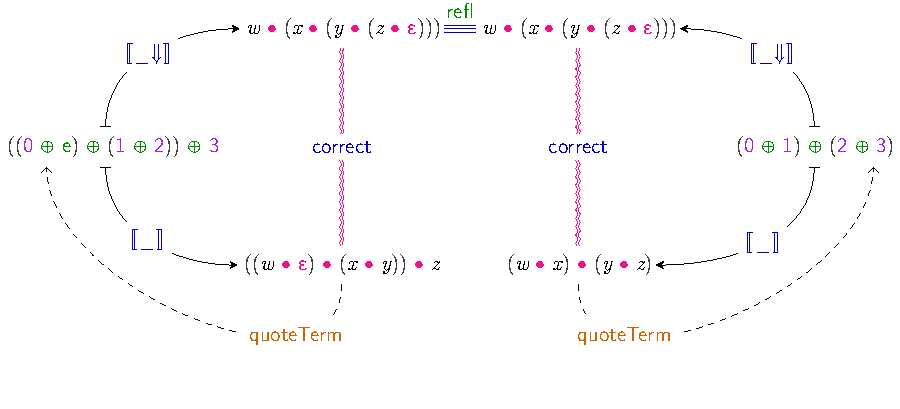
\includegraphics[draft=false]{graphics/reflexive-process}
  }
  \caption{The Reflexive Proof Process}
  \label{proof-process}
\end{figure*}
Now we have a concrete way to link the normalized and non-normalized forms of
the expressions. A diagram of the strategy for constructing our proof is in
figure~\ref{proof-process}. The goal is to construct a proof of equivalence
between the two expressions at the bottom: to do this, we first construct the
ASTs which represent the two expressions (for now, we'll assume the user
constructs this AST themselves. Later we'll see how to construct it
automatically from the provided expressions). In figure~\ref{proof-process},
these ASTs are on the far left and right. Then, we can evaluate it into either
the normalized form (\(\AgdaFunction{⟦\_⇓⟧}\)), or the unnormalized
form(\(\AgdaFunction{⟦\_⟧}\)). Since the normalized forms are syntactically
equal, all we need is \(\AgdaInductiveConstructor{refl}\) to prove their
equality. The only missing part now is \(\AgdaFunction{correct}\).

Taking the non-normalizing interpreter as a template, the three cases
\(\AgdaFunction{correct}\) will have to deal with are as follows\footnotemark:
\begin{align}
  \AgdaFunction{⟦} \; x \; \AgdaInductiveConstructor{⊕} \; y \; \AgdaFunction{⟧} \; \rho \; &\AgdaField{≈} \; \AgdaFunction{⟦} \; x \; \AgdaInductiveConstructor{⊕} \; y \; \AgdaFunction{⇓⟧} \; \rho \label{plus-hom} \\
  \AgdaFunction{⟦}      \; \AgdaInductiveConstructor{e}      \; \AgdaFunction{⟧} \; \rho \; &\AgdaField{≈} \; \AgdaFunction{⟦}      \; \AgdaInductiveConstructor{e}      \; \AgdaFunction{⇓⟧} \; \rho \label{e-hom}    \\
  \AgdaFunction{⟦}      \; \AgdaInductiveConstructor{ν} \; i \; \AgdaFunction{⟧} \; \rho \; &\AgdaField{≈} \; \AgdaFunction{⟦}      \; \AgdaInductiveConstructor{ν} \; i \; \AgdaFunction{⇓⟧} \; \rho \label{var-hom}
\end{align}
\footnotetext{
  Equations \ref{plus-hom} and \ref{e-hom} comprise a monoid
  homomorphism.
}

Proving each of these cases in turn finally verifies the correctness of our list
language.
\ExecuteMetaData[Monoids.tex]{correct-ast}
\subsection{Usage}
Combining all of the components above, with some plumbing provided by the
\(\AgdaModule{Relation.Binary.Reflection}\) module, we can finally automate the
solving of the original identity: figure~\ref{mon-auto-proof}.
\begin{figure}
  \ExecuteMetaData[Monoids.tex]{ident-auto-proof}
  \caption{Automated Proof of the Identity in figure~\ref{mon-ident}}
  \label{mon-auto-proof}
\end{figure}
\subsubsection{Reflection}
While the procedure is now automated, the interface isn't ideal: users have to
write the identity they want to prove \emph{and} the AST representing the
identity. Removing this step is the job of reflection
(section~\ref{reflection}): in figure~\ref{proof-process} it's represented by
the path labeled \(\AgdaKeyword{quoteTerm}\).
\section{A Polynomial Solver}
With the monoid solver as a template, the components required for the ring
solver are as follows: a normal form, a concrete representation of
expressions, and a proof of correctness (homomorphism). Before addressing each
of these, a small digression.
\subsection{Choice of Algebra}
So far, we've assumed the solver is defined over commutative rings. That wasn't
the only algebra available to us when writing a solver, though: we've
demonstrated techniques using monoids in the previous section, and
indeed\cite{geuvers_automatically_2017} uses \emph{non}commutative rings as its
algebra. Here, we will justify our\footnotemark choice (and admit to a minor lie).
\footnotetext{
  ``Our'' choice here is the same choice as in\cite{gregoire_proving_2005}.
}

Because we want to solve arithmetic equations, we will need the basic operations
of addition, multiplication, subtraction, and exponentiation (to a power in
\(\mathbb{N}\)). This is only half of the story, though: along with those
operations we will need to specify the laws or equations that they obey
(commutativity, associativity, etc.). Here we must strike a balance: the more
equations specified, the more equalities the solver can prove, but the fewer
types the solver will be available for.

The elephant in the room here is \(\mathbb{N}\): perhaps the most used numeric
type in Agda, it doesn't have an additive inverse. So that our solver will still
function with it as a carrier type, we don't require
\[x - x = 0\]
to hold. This lets us lawfully define negation as the identity function for
\(\mathbb{N}\).

A potential worry is that because we don't require \(x - x = 0\)
axiomatically, it won't be provable in our system. This is not so: as is pointed
out in\cite{gregoire_proving_2005},as long as \(1 - 1\) reduces to \(0\) in the
coefficient set, the solver will verify the identity.
\subsection{Horner Normal Form}
The free representation of polynomials we choose is a list of coefficients,
least significant first (``Horner Normal Form''). Our initial attempt at
encoding this representation will begin like so:
\ExecuteMetaData[HornerNormalForm.tex]{opening}
The entire module is parameterized by the choice of coefficient. This
coefficient should support the ring operations, but it is ``raw'', i.e. it
doesn't prove the ring laws. The operations\footnotemark on the polynomial
itself are defined in figure~\ref{simple-ops}.
\footnotetext{
  Symbols chosen for operators use the following mnemonic:
  \begin{enumerate}
    \item Operators preceded with ``\(\mathbb{N}.\)'' are defined over
      \(\mathbb{N}\); e.g. \(\mathbb{N}.+\), \(\mathbb{N}.*\).
    \item Plain operators, like \(+\) and \(*\), are defined over the
      coefficients.
    \item Boxed operators, like \(\boxplus\) and \(\boxtimes\), are defined over
      polynomials.
  \end{enumerate}
}

\begin{figure}
  \ExecuteMetaData[HornerNormalForm.tex]{impl}
  \caption{
    Simple Operations on Dense Horner Normal Form}
  \label{simple-ops}
\end{figure}
Finally, evaluation of the polynomial uses Horner's rule to minimize
multiplications:
\ExecuteMetaData[HornerNormalForm.tex]{eval}
\subsection{Eliminating Redundancy}
As it stands, the above representation has two problems:

\begin{description}
  \item[Redundancy] We allow trailing zeroes, so the polynomial $2x$ could be
    represented by any of the following:
  
    \begin{align*}
      & 0, 2 \\
      & 0, 2, 0 \\
      & 0, 2, 0, 0 \\
      & 0, 2, 0, 0, 0, 0, 0
    \end{align*}
    
    This redundancy means that we don't truly have a canonical form.
  \item[Inefficiency] Expressions will tend to have large gaps, full only of
    zeroes. Something like $x^5$ will be represented as a list with 6 elements,
    only the last one being of interest. Since addition is linear in the length
    of the list, and multiplication quadratic, this is a major concern.
\end{description}
Since both leading and trailing zeroes present a problem, we will disallow
zeroes altogether. Instead, like in\cite{gregoire_proving_2005}, we will store a
``power index'' with every coefficient\footnotemark. This index represents the
``distance to the next non-zero coefficient''.
\footnotetext{
  In\cite{gregoire_proving_2005}, the expression \((c , i) \squaredots P\)
  represents \(P \times X^i + c\). We found that \(X^i \times (c + X \times P)\)
  is a more natural translation, and it's what we use here. A power index of
  \(i\) in this representation is equivalent to a power index of \(i+1\)
  in\cite{gregoire_proving_2005}.
}

As an example, the polynomial:
\[ 3 + 2x^2 + 4x^5 + 2x^7 \]
Will be represented as:
\[ (3,0),(2,1),(4,2),(2,1) \]
Or, mathematically:
\[ x^0 (3 + x x^1 (2 + x x^2 * (4 + x x^1 (2 + x 0)))) \]

\begin{definition}[Dense and Sparse Encodings]
  In situations like this, where inductive types have large ``gaps'' of
  zero-like terms between interesting (non-zero-like) terms, the encoding which
  uses an index to represent the size of the gap to the next interesting term
  will be called \emph{sparse}, and the encoding which simply stores the zero
  terms will be called \emph{dense}.
\end{definition}

Now that we have chosen a normal form (polynomials without 0), can we prove that
our implementation always maintains it? In \cite{gregoire_proving_2005}, care
is taken to ensure all operations include a normalizing step, but this is not
verified: here, we do exactly that.

To check for zero, we require the user supply a decidable predicate on the
coefficients. This changes the module declaration like so:
\ExecuteMetaData[EliminatingRedundancy.tex]{opening}

Importantly, we don't require that the user provides a decidable proof of
\emph{equivalence}, rather just a decidable proof of some predicate which can
later be translated into an equivalence with zero. Functionally, this means the
user could supply a predicate which is always false, or a predicate which is
only \emph{weakly} decidable.

And now we have a definition for sparse polynomials:
\ExecuteMetaData[EliminatingRedundancy.tex]{decl}

The proof of nonzero is marked irrelevant (by preceding it with a dot) to avoid
computing it at runtime.

We can wrap up the implementation with a cleaner interface by providing a
normalizing version of \(\AgdaInductiveConstructor{\_∷\_}\):
\ExecuteMetaData[EliminatingRedundancy.tex]{norm-cons}
\subsection{Multiple Variables}
So far, the polynomials have been (suspiciously) single-variable. Luckily,
there's a natural way to add multiple variables: nesting. For a polynomial with
one variable (\(x\), say), the implementation is as before. For \emph{two}
variables (\(x\) and \(y\)), we will have an outer polynomial in \(y\), whose
\emph{coefficients} are polynomials in \(x\). Put inductively, a polynomial with
0 variables is simply a coefficient; a polynomial with $n$ variables is a list
of polynomials with $n-1$ variables. In types:
\ExecuteMetaData[SparseMulti.tex]{dense-poly} 
\subsection{Efficiency in Indexed Types}
\subsubsection{Call-Pattern Specialization}
While both sparse encodings provide a more space-efficient representation, the
computational efficiency has yet to be realized. Starting with the sparse
monomial, we'll look at the addition function. In the dense encoding
(figure~\ref{simple-ops}), we needed to line up corresponding coefficients to
add together. For this encoding, the ``corresponding'' coefficients are slightly
harder to find. In order to line things p correctly, we'll need to compare the
gap indices. This, however, presents our first problem:
\ExecuteMetaData[EliminatingRedundancy.tex]{nonterm-add}
It doesn't pass the termination checker! While it does indeed terminate, it
isn't structurally decreasing in its arguments. To make it structurally
decreasing, and therefore show the compiler it terminates, we'll use a
well-known optimization for functional languages called ``call-pattern
specialization''\cite{jones_call-pattern_2007}.
\begin{principle}[To make termination obvious, perform call-pattern
    specialization]
  Unpack any constructors into function arguments as soon as possible, and
  eliminate any redundant pattern matches in the offending functions. Happily,
  this transformation both makes termination more obvious \emph{and} improves
  performance.

  GHC automatically performs this optimization: perhaps Agda's compiler could do
  something similar to reveal more terminating programs.
\end{principle}

For our case, the principle applied can be seen in figure~\ref{term-add}.

\begin{figure*}
  \centering
  \ExecuteMetaData[EliminatingRedundancy.tex]{term-add}
  \caption{Termination by Call-Pattern Specialization}
  \label{term-add}
\end{figure*}

\subsubsection{Built-In Functions}
\begin{figure}
  \ExecuteMetaData[EfficiencyInIndexedTypes.tex]{ord-type}
  \caption{The Ordering Indexed Type}
  \label{ord-type}
\end{figure}
The second optimization we might rely on involves the call to
\(\AgdaFunction{compare}\). This is a classic ``leftist'' function: it returns
an \emph{indexed} data type (figure~\ref{ord-type}). The compare function itself
is \(\mathcal{O}(\min(n, m))\):

\ExecuteMetaData[EfficiencyInIndexedTypes.tex]{cmp-impl}

The implementation of \(\AgdaFunction{compare}\) may raise suspicion with
regards to efficiency: if this encoding of polynomials improves time complexity
by skipping the gaps, don't we lose all of that when we encode the gaps as Peano
numbers?

The answer is a tentative no. Firstly, since we are comparing gaps, the
complexity can be no larger than that of the dense implementation. Secondly, the
operations we're most concerned about are those on the underlying coefficient;
and, indeed, this sparse encoding does reduce the number of those significantly.
Thirdly, if a fast implementation of \(\AgdaFunction{compare}\) is really and
truly demanded, there are tricks we can employ.

Agda has a number of built-in functions on the natural numbers: when applied to
closed terms, these call to an implementation on Haskell's \texttt{Integer}
type, rather than the unary implementation. For our uses, the functions of
interest are \(\AgdaFunction{-}\), \(\AgdaFunction{+}\), \(\AgdaFunction{<}\),
and \(\AgdaFunction{==}\). The comparison functions provide booleans rather than
evidence, but we can prove they correspond to the evidence-providing versions:
\ExecuteMetaData[EfficiencyInIndexedTypes.tex]{fast-cmp-hom}
Combined with judicious use of \(\AgdaFunction{erase}\) and
\(\AgdaFunction{inspect}\), we get the implementation in figure~\ref{fast-cmp}.

\begin{figure*}
  \centering
  \ExecuteMetaData[EfficiencyInIndexedTypes.tex]{fast-cmp}
  \caption{Fast comparison function using built-in functions on the natural
    numbers}
  \label{fast-cmp}
\end{figure*}
\subsubsection{Unification}
The way we added the capability for multiple variables to our polynomial type
actually introduced an opportunity for another sparse encoding.

In a polynomial of $n$ variables, addressing the $n^{th}$ variable needlessly
requires $n-1$ layers of nesting. Alternatively, a constant expression in this
polynomial is hidden behind $n$ layers of nesting.

In contrast to the previous sparse encoding, though, the size of the gap is
type-relevant. Because of this, the gap will have to be lifted into an index
(figure~\ref{sparse-poly}).

\begin{figure}
  \ExecuteMetaData[SparseMulti.tex]{sparse-poly}
  \caption{A Sparse Multivariate Polynomial}
  \label{sparse-poly}
\end{figure}

It encodes ``less than'' in the same way that the ordering type did
(figure~\ref{ord-type}), so it may seem (initially) like a perfect fit. However,
we run into issues when it comes to performing the comparison-like operations
above. Because it's an indexed type, pattern matching on it will force
unification of the index with whatever type variable it was bound to. This is
problematic because the index is defined by a function: pattern match on a pair
of \(\AgdaDatatype{Poly}\)s and you're asking Agda to unify \(i_1 + j_1\) and
\(i_2 + j_2\), a task it will likely find too difficult. How do we avoid this?
\begin{principle}[Don't touch the green slime]
  When combining prescriptive and descriptive indices, ensure both are in
  constructor form. Exclude defined functions which yield difficult unification
  problems\cite{mcbride_polynomial_2018}.
\end{principle}
We'll have to take another route.
\subsubsection{Hanging Indices}
First, we'll redefine our polynomial like so:
\ExecuteMetaData[EfficiencyInIndexedTypes.tex]{sparse-poly}
The type is now parameterized, rather than indexed: our pattern-matching woes
have been solved. Also, instead of storing the gap explicitly, we store a proof
that the nested polynomial has no more variables then the outer.

The choice of definition for this proof has important performance implications,
as the proof will need to mesh with whatever comparison function we use for the
injection indices. The Agda standard library\cite{danielsson_agda_2018} gives us
3 options.
\begin{description}
  \item[Option 1: The Standard Way] The most commonly used definition of
    \(\leq\) is as follows:
    \ExecuteMetaData[EfficiencyInIndexedTypes.tex]{leq-1}
    Trying to proceed with this type will yield a nasty performance bug, though:
    the inductive structure of the type gives us no real information about the
    underlying ``gap'', so we're forced to compare the actual size of the
    nested polynomials. To see why this is a problem, consider the following
    sequence of nestings:

    \[ (5 ≤ 6), (4 ≤ 5), (3 ≤ 4), (1 ≤ 3), (0 ≤ 1) \]

    The outer polynomial has 6 variables, but it has a gap to its inner
    polynomial of 5, and so on. The comparisons will be made on 5, 4, 3, 1, and
    0. Like repeatedly taking the length of the tail of a list, this is
    quadratic.
  \item[Option 2: With Propositional Equality] Once you realize we need to be
    comparing the gaps and not the tails, another encoding of \(\leq\) in
    Data.Nat seems the best option:
    \ExecuteMetaData[EfficiencyInIndexedTypes.tex]{leq-2}
    It stores the gap \emph{right there}: in \(\AgdaField{k}\)!

    Unfortunately, though, we're still stuck. While you can indeed run your
    comparison on \(k\), you're not left with much information about the rest.
    Say, for instance, you find out that two respective \(\AgdaField{k}\)s are
    equal. What about the \(m\)s? Of course, you \emph{can} show that they must
    be equal as well, but it requires a proof. Similarly in the less-than or
    greater-than cases: each time, you need to show that the information about
    \(\AgdaField{k}\) corresponds to information about \(m\). Again, all of this
    can be done, but it all requires propositional proofs, which are messy, and
    slow. Erasure is an option, but I'm not sure of the correctness of that
    approach.
  \item[Option 3] What we really want is to \emph{run} the comparison function
    on the gap, but get the result on the tail. Turns out we can do exactly that
    with the following:
    \ExecuteMetaData[EfficiencyInIndexedTypes.tex]{leq-3}
    This is the structure we will choose.
\end{description}
What's important about our chosen type is that, ignoring the indices, its
inductive structure mimics that of the actual Peano encoding of the gaps
previously. In other words, \(\AgdaInductiveConstructor{m≤m}\) appears wherever
\(\AgdaInductiveConstructor{zero}\) would have previously, and
\(\AgdaInductiveConstructor{≤-s}\) where there was
\(\AgdaInductiveConstructor{suc}\). This gives us another principle:
\begin{principle}[To add more type information, to a type or function, keep the
  \emph{structure} of the old type, while \emph{hanging} new information off of it]
  The three options above each present avenues to possible solutions to our
  ``gap'' problem, but they should have been ignored. Instead, we should have
  taken the previous untyped solution, and seen where in the inductive cases of
  the types used extra type information could have been stored. With this
  approach, the efficiency of the already-written algorithms is maintained. This
  practice can be somewhat automated using
  \emph{ornaments}\cite{dagand_essence_2017}.
\end{principle}

This is not yet enough to fully write our comparison function, though. Looking
back to the previous definition of \(\AgdaDatatype{Ordering}\), we see that it
contains \(\AgdaFunction{+}\); we need an equivalent function on
\(\AgdaDatatype{≤}\). Remember that the quantity we'll be adding is adjacent
gaps: this suggests the equivalent function is \emph{transitivity}:
\ExecuteMetaData[EfficiencyInIndexedTypes.tex]{leq-trans}
And with that, we have enough to define our comparison function:
\ExecuteMetaData[EfficiencyInIndexedTypes.tex]{leq-compare}
\subsection{Abstraction and Folds for Simpler Proofs}
At this point, following our many optimizations, the task of proving
homomorphism for these implementations is more than a little daunting. However,
we can ease the burden somewhat by leveraging the \(\AgdaFunction{foldr}\)
function, in a similar way to\cite{mu_algebra_2009}.

The goal is to modularize the proofs by independently proving the correctness of
each optimization. To do this, we will strive to write the arithmetic operations
as higher-order functions, which operate over the ``unoptimized'' version of the
polynomials (the dense versions), and have an intermediate function convert to
and from the dense encoding. As a case study, we'll work with the negation
function. Our initial definition (on the type defined in
figure~\ref{final-poly-def}) is as follows:

\ExecuteMetaData[AbstractionAndFolds.tex]{simple}

Immediately we can recognize two functions which are good candidates for
separated homomorphism proofs: \(\AgdaFunction{∷↓}\) and \(\AgdaFunction{Π↓}\).
These functions will be used in every arithmetic operation, so it stands to
reason that a separate proof of their correctness should save us some
repetition. The lemmas are as follows:

\ExecuteMetaData[AbstractionAndFolds.tex]{lemmas}

Next, the \(\AgdaFunction{go}\) helper function is an obvious candidate for
\(\AgdaFunction{foldr}\)\footnotemark.

\footnotetext{Using \(\AgdaFunction{foldr}\) will actually yield some
  termination problems, which we will have to deal with in the next section}.

\ExecuteMetaData[AbstractionAndFolds.tex]{with-foldr}

Continuing in this vein, we are able to isolate the component of this function
which is different from the other operations, and therefore confine our proofs
to that difference. In this particular case, we use the following lemma:

\ExecuteMetaData[AbstractionAndFolds.tex]{poly-mapR}

In this way, we demonstrate a concrete and practical use
of\cite{mu_algebra_2009}. \todo{Expand!}
\subsection{Proving Higher-Order Termination With Well-Founded Recursion}
Unfortunately, by using a higher-order function, we've obscured the fact that
the negation operation obviously terminates.

To prove it, we'll use \emph{well-founded
  recursion}\cite{nordstrom_terminating_1987}. It works by providing a relation
which describes some strictly decreasing finite chain: \(<\) on \(\mathbb{N}\),
for instance. It's strictly decreasing because the first argument always gets
smaller (in contrast to, say, \(\leq\)), and it's finite because it must end at
0.

In Agda,  well-founded recursion is specified with the following type:
\ExecuteMetaData[AbstractionAndFolds.tex]{acc-def}

Agda's termination checker algorithm comes from foetus\cite{abel_foetus_1998}:
it's relatively simple, and relies on \emph{structural termination}. Take the
following function:
\[ \AgdaFunction{f} \; x = \AgdaNumber{1} \; \AgdaFunction{+} \;
  \AgdaFunction{f} \; y \]

Agda will determine \(\AgdaFunction{f}\) to be terminating if and only if \(y\)
is \emph{structurally smaller} than \(x\). In practice, this means that \(y\)
needs to be a subnode of \(x\)'s recursive structure. For instance (ignoring
partiality for now), all of the following are allowed:
\begin{align*}
\AgdaFunction{f} \; (\AgdaInductiveConstructor{suc} \; y)     &= \AgdaFunction{f} \; y \\
\AgdaFunction{f} \; (\_ \; \AgdaInductiveConstructor{∷} \; y) &= \AgdaFunction{f} \; y
\end{align*}

Crucially, no matter how many arguments \(\AgdaFunction{f}\) has, if any one of
them is structurally decreasing, it will pass the termination checker. This is
where \(\AgdaDatatype{Acc}\) comes in: as far as Agda is concerned, whatever's
returned by the function stored in \(\AgdaDatatype{Acc}\) is structurally
smaller that the outer type it was wrapped in. So you can add it as a parameter
to the dangerous functions, and call the wrapped function to generate the new
\(\AgdaDatatype{Acc}\) to pass to the recursive call.

Of course, to \emph{call} the function you have to supply it with an argument: a
proof that the relation holds. This part is why well-founded recursion is valid:
whoever constructed the \(\AgdaDatatype{Acc}\) originally will have had to pass
the termination checker. In other words, they will have written a recursive
function to generate nested \(\AgdaDatatype{Acc}\)s, where the only argument to
that function is the relation. In this way, we have moved the obligation of
proving termination from the call-site to the construction site. For the
relation we use, the construction function for \(\AgdaDatatype{Acc}\) is as
follows:

\ExecuteMetaData[AbstractionAndFolds.tex]{acc-impl}

One of the warts of well-founded recursion is that usually the programmer has to
separately construct the relation they're interested in. As well as being
complex, it can be computationally expensive. Usually the compiler can elide the
calls, recognizing that the argument isn't used, but the optimization can't be
guaranteed.

Luckily, in our case, the relation is already lying around, in the injection
index. So we can just use that!
\ExecuteMetaData[AbstractionAndFolds.tex]{terminating}

\section{Reflection} \label{reflection}
One annoyance of the automated solver is that we have to write the expression we
want to solve twice: once in the type signature, and again in the argument
supplied to solve. See figure~\ref{mon-auto-proof} for an example of this kind
of duplication. We can cut down on the writing we need to do by half by omitting
the type signature, but for a user, this is the \emph{wrong half}: the syntax
and structure of the AST is something of an implementation detail, and is not
something we should require the user to learn. Instead, we provide the following
interface:
\ExecuteMetaData[ReflectionSection.tex]{refl-lemma}

The call to \(\AgdaMacro{solve}\) first infers the goal type, then constructs
the corresponding AST to hand to the solver. Interestingly, the goal type need
not be provided explicitly: if a user has a type mismatch between two
expressions, just sticking in a call to \(\AgdaMacro{solve}\) in the appropriate
place will often fix the problem. Furthermore, by not explicitly writing the AST
in the program's source code, functions become more extensible and resilient to
minor changes. As long as the two expressions match up semantically, rather than
syntactically, the solver will figure it out.

We build this interface using Agda's reflection
mechanisms\cite{van_der_walt_reflection_2012}. Reflection in Agda allows a
program to inspect and modify its own code. There are three basic components
that we'll use for the reflection machinery:
\begin{description}
  \item[\(\AgdaDatatype{Term}\)] The representation of Agda's AST, retrievable
    via \(\AgdaKeyword{quoteTerm}\).
  \item[\(\AgdaDatatype{Name}\)] The representation of identifiers, retrievable
    via \(\AgdaKeyword{quote}\).
  \item[\(\AgdaDatatype{TC}\)] The type-checker monad, which includes scoping
    and environment information, can raise type errors, unify variables, or
    provide fresh names. Computations in the \(\AgdaDatatype{TC}\) monad can be
    run with \(\AgdaKeyword{unquote}\).
\end{description}

While \(\AgdaKeyword{quote}\), \(\AgdaKeyword{quoteTerm}\), and
\(\AgdaKeyword{unquote}\) provide all the functionality we need, they're
somewhat low-level, so instead we will define \emph{macros}. Macros (in Agda)
are essentially syntactic sugar for the above keywords. They're defined by first
declaring a \(\AgdaKeyword{macro}\) block, and then defining a function within
it which has the return type:
\ExecuteMetaData[ReflectionSection.tex]{return-type}

The rest of the arguments can be treated normally like any other function, or,
if they have the type \(\AgdaDatatype{Term}\) or \(\AgdaDatatype{Name}\),
they're quoted before being passed in. The final argument to the function is the
hole representing where the macro was called: to ``return'' a value you unify
it with that hole. As an example, here's a macro to count the number of
occurrences of some identifier in an expression:
\ExecuteMetaData[ReflectionSection.tex]{occ-of}

Some of the core characteristics of working with the reflected AST are clear
here. Firstly, it's verbose. The \(\AgdaFunction{natTerm}\) function, for
instance, simply gets the syntactic representation of a natural number.
Unfortunately, we can't necessarily just call \(\AgdaKeyword{quoteTerm}\): the
returned AST includes all kinds of information about context and environment
which can clash with the environment where the macro is instantiated. A large
amount of reflection and metaprogramming in Agda unfortunately consists of this
kind of boilerplate (currently, at any rate).

Next, it's far less \emph{typed} than it could be. To be clear, it doesn't break
type safety: the generated program is still type-checked, but you can generate
code with a type error in it without any difficulty. On the other end, the
reflected AST doesn't contain as much type information as it could, which is
often an annoyance. 

Finally, it's fragile. Say we want to solve some expression in
\(\AgdaDatatype{ℕ}\). Converting this to some \(\AgdaDatatype{Expr}\) type will
involve, among other things, being able to find functions like
\(\AgdaFunction{+}\) and \(\AgdaFunction{*}\) in the expression. However, if the
user implements \(\AgdaDatatype{AlmostCommutativeRing}\) in the normal way,
there'll be two identifiers which refer to each of those functions: one being
the original implementation in \(\AgdaModule{Data.Nat}\), and the other being
the field in \(\AgdaDatatype{AlmostCommutativeRing}\). But wait, it gets worse:
in actual fact, there may well be \emph{three} identifiers. Remember that the
``almost'' qualifier in \(\AgdaDatatype{AlmostCommutativeRing}\) refers to the
fact that negation isn't required to cancel, allowing us to use types without a
notion of negation (like  \(\AgdaDatatype{ℕ}\)). With the best of intentions, we
may even provide a helper function which takes a \(\AgdaDatatype{Semiring}\)
(ring without negation) and converts it into a
\(\AgdaDatatype{AlmostCommutativeRing}\), supplying the identity function for
negation. That's where our third identifier comes from: the
\(\AgdaDatatype{Semiring}\) type. The third identifier is the field in the
\(\AgdaDatatype{Semiring}\) record. If the \(\AgdaDatatype{Semiring}\) record is
constructed from other records again (two monoids, say), we get even more
identifiers to choose from.

This all makes it difficult to check if a function application is
\(\AgdaFunction{+}\), because we're only going to look at name equality. The
following, for example, is morally the same as the argument to
\(\AgdaMacro{occPlus}\) above, but returns a different argument, because we use
an aliased version of \(\AgdaFunction{+}\):
\ExecuteMetaData[ReflectionSection.tex]{occ-wrong}

So our solver will demand that the user only refer to the functions defined in
the record.

Something that isn't visible in the example above the fact that
\(\AgdaDatatype{Term}\) uses de Bruijn indices for variables. This means we have
to be extra careful about scope.

\subsection{Building The AST for Proving}
Though \(\AgdaDatatype{Term}\) is itself an AST we could theoretically
manipulate and use in the prover, as is demonstrated above it's complex and
unwieldy: what we really want is to use a smaller AST for ring expressions, like
the one for lists.
\ExecuteMetaData[ReflectionSection.tex]{expr-def}

To that end, we'll need build the \(\AgdaDatatype{Term}\) which will construct
it for us.

First, to make things easier on ourselves, we'll define some pattern synonyms:
\ExecuteMetaData[ReflectionSection.tex]{synonyms}

These match visible and hidden arguments, respectively.

Next, we'll need another helper which applies the hidden arguments to the
constructors for \(\AgdaDatatype{Expr}\). There are \emph{three} of these. The
first is the universe level, the second is the Carrier type, and the third is
the number of variables it's indexed by.
\ExecuteMetaData[ReflectionSection.tex]{expr-hidden}
The \(\AgdaInductiveConstructor{unknown}\) value translates into using an
underscore; it means we're asking Agda to infer the value in its place. This
might seem suboptimal: we can probably figure out the values of those
underscores, so shouldn't we try and find them, and supply them instead? In our
experience, the answer is no.

\begin{principle}[Don't help the compiler]
  Supply the \emph{minimal} amount of information possible in the AST to be
  unquoted, relying on inference as much as possible. The metalanguage is
  fragile and finicky with regards to scopes and context: the compiler isn't.
  You're more likely to get an argument wrong if you try and figure it out than
  the compiler is.
\end{principle}

Using this, we can make a function for the AST which will generate a constant
expression:
\ExecuteMetaData[ReflectionSection.tex]{expr-const-ast}
\subsection{Matching on the Reflected Expression}
There are three components we want to match on in the reflected expression: ring
operators, variables, and constants.
\subsubsection{Matching the Ring Operators}
We'll do this via name equality. The three names we're interested in are as
follows:
\ExecuteMetaData[ReflectionSection]{op-names}
When we encounter the AST constructor which corresponds to a name reference
\(\AgdaInductiveConstructor{def}\), we test for equality on each of these names
successively. When (if) we get a match, we call one of the following functions,
depending on the operator's arity:
\ExecuteMetaData[ReflectionSection.tex]{op-build}

These take a list of arguments, dropping any extra from the front, and package
up the relevant ones with the relevant constructor from the AST. It may seem
strange that there are ``extra'' arguments: surely these operators should have
the same number of arguments as their arity?

\begin{principle}[Don't assume structure]
  Details like the order or number of implicit arguments to a function often
  can't be relied upon: be accommodating in your matching functions, only
  extracting components you really and truly need. In this case, for instance,
  the first argument will actually be the
  \(\AgdaDatatype{AlmostCommutativeRing}\) record, as these functions are
  actually field accessors. But wait, no it won't---the first argument will
  actually be the hidden universe level of the carrier type, and the second
  (also hidden) will be the universe level of the equality relation. Only the
  third is the record, making the following arguments the ``real'' arguments to
  the function. Remember, none of this is typed, so if something changes in the
  order of arguments, you'll get type errors where you call
  \(\AgdaMacro{solve}\), not where it's implemented.
\end{principle}
\subsubsection{Matching Variables}
This task is actually reasonably simple: we check the de Bruijn index of the
variable question, and if it's smaller than the number of variables in the ring
expression, we simply leave it as is. We can do this because we're using the
interface provided by \(\AgdaModule{Relation.Binary.Reflection}\) as an
intermediary: it will wrap up the variables in our \(\AgdaDatatype{Expr}\) for
us automatically. Which leads us to another observation:
\begin{principle}[Try and implement as much of the logic outside of reflection
    as possible]
  The expressive power granted by reflection comes with poor error messages,
  fragility, and a loss of first-class status. If something can be done without
  reflection, \emph{do it}, and use reflection as the glue to get from one
  standard representation to another.
\end{principle}
\subsubsection{Matching Constants}
This task seems the most daunting: with all of the logic we required before just
to match expressions, how are we going to match the carrier type? Do we need the
user to provide that function? Some kind of matching logic (as
in\cite{jedynak_simple_2018}), which would need to recognize every constructor
case, and build the corresponding \(\AgdaDatatype{Term}\)?

Maybe we go another direction: we could search the subexpression to see if it
contains any free variables, and decide based on that. \(\mathcal{O}(n^2)\)
time, anyone?

If the reflection API was different, this task could conceivably be made easier:
for now, what most people seem to do is automate the process (as
in\cite{norell_agda-prelude_2018}).

It is only by a very lucky coincidence that we can avoid all of this. Notice
that all of the other cases are spoken for: in a correctly constructed
expression, if no other clause matches, then what's left \emph{has} to be a
constant. So we just wrap it up in the constant constructor!

\resetlinenumber[1]

\begin{linenumbers}
\ExecuteMetaData[ReflectionSection.tex]{to-expr}
\end{linenumbers}

You'll notice that in the clauses where we fail to find a match (lines 8, 11,
and 12), we assume that what we must have is a constant, so we just wrap it up
as if it were one. 

But what about incorrectly constructed expressions? What if the user makes a
mistake in what they ask us to solve: surely we can't \emph{assume} correctness?
Well actually:

\begin{principle}[Ask for forgiveness, not permission]
  If the input to your macro requires the user to write an expression which
  conforms to a certain structure, \emph{assume} that they have done so; don't
  check for it and proceed conditionally. With careful structuring of the
  macro's output, you can funnel the type error to exactly where the user was
  incorrect. For instance, in this case, if the user makes a mistake and the
  subexpression isn't a constant \(\AgdaDatatype{Carrier}\), the type error
  they'll get back will be something like ``Expected type
  \(\AgdaDatatype{Carrier}\), found ...''. In other words, exactly the type
  error we expect!
\end{principle}

\subsection{Building the Solution}
The rest of the function is similar to above. Eventually, it will call
\(\AgdaModule{Relation.Binary.Reflection}\) with the constructed arguments.
Because we've been careful not to supply any type information we don't need to,
we actually get decent error messages when the solver fails. For instance, if we
ask it to solve the following:

\ExecuteMetaData[ReflectionSection.tex]{wrong-lemma}

It will demonstrate where exactly it fails, with the error message:

\[
 (y \; \AgdaFunction{+} \; \AgdaNumber{0} \; \AgdaFunction{*} \; y) \;
 \AgdaFunction{*} \;
 \AgdaNumber{1} \neq x
\]

This is because we pass it \(\AgdaField{refl}\) as the proof that the normal
forms are equal: if they're not, this is where we'll get an error.
\section{Setoid Applications} \label{equivalence}
After constraining ourselves by only demanding a setoid from the user, we now
get to reap some rather interesting benefits.
\subsection{Isomorphisms}
The first, and most obvious, ``exotic'' setoid is that over a universe of types.
The relation is an \emph{isomorphism} between these types. In this way, the
solver can now automatically construct functions to convert between equivalent
types. This has been explored before in a number of settings.
\subsection{Pedagogical Solutions} \todo{Expand!}
One of the most widely-used and successful applications of computer algebra,
especially among non-programmers, has been Wolfram
Alpha\cite{wolfram_research_inc._wolframalpha_2019}. Perhaps its most used
feature is pedagogical (or pedagogic) solutions to maths
problems\cite{the_development_team_step-by-step_2009}. For instance, given the
input \(x^2 + 5 x + 6 = 0\), it will give the following output:

\begin{align*}
  x^2 + 5x + 6   = 0 \\
  (x + 2)(x + 3) = 0 \\
  x + 2 = 0   \; \text{or} \; x + 3 = 0 \\
  x     = -2  \; \text{or} \; x + 2 = 0 \\
  x     = -2  \; \text{or} \; x     = -3
\end{align*}

These tools can be invaluable for students learning basic mathematics.
Unfortunately, much of the software capable of generating usable solutions is
proprietary, and little information is available as to their implementation
techniques.\cite{lioubartsev_constructing_2016} is perhaps the best current work
on the topic, but even so very little exists in the way of the theoretical basis
for pedagogical solutions.

Taking\cite{lioubartsev_constructing_2016} as a jumping-off point, we can see
that solutions are treated as \emph{paths}: indeed, A* is the underlying
algorithm used.

These paths have edges of rewrite rules---``commutativity of addition'', etc.
The vertices are equation states, and the start and end points of the path are
the left-hand-side and right-hand-side of the equation, respectively. It's clear
that we can form from this a relation with symmetry, transitivity and
reflexivity: enough to satisfy our solver.

\section{The Correct-By-Construction Approach}
The Agda and Coq communities exhibit something of a cultural difference when it
comes to proving things. Coq users seem to prefer writing simpler, almost
non-dependent code and algorithms, to separately prove properties about that
code in auxiliary lemmas. Agda users, on the other hand, seem to prefer baking
the properties into the definition of the types themselves, and writing the
functions in such a way that they prove those properties as they go (the
``correct-by-construction'' approach).

There are advantages and disadvantages to each. The Coq approach, for instance,
allows you to reuse the same functions in different settings, verifying
different properties about them depending on what's required. In Agda, this is
more difficult: you usually need a new type for every invariant you maintain
(lists, and then length-indexed lists, and then sorted lists, etc.). On the
other hand, the proofs themselves often contain a lot of duplication of the
logic in the implementation: in the Agda style, you avoid this duplication, by
doing both at once. Also worth noting is that occasionally attempting to write a
function that is correct by construction will lead to a much more elegant
formulation of the original algorithm, or expose symmetries between the proof
and implementation that would have been difficult to see otherwise.

\cite{gregoire_proving_2005}, as an example, is very much in the Coq style: the
definition of the polynomial type has no type indices, and makes no requirements
on its internal structure:
\begin{small}
\begin{verbatim}
Inductive Pol (C:Set) : Set :=
  | Pc : C -> Pol C
  | Pinj : positive -> Pol C -> Pol C
  | PX : Pol C -> positive -> Pol C -> Pol C.
\end{verbatim}
\end{small}

The implementation presented here straddles both camps: we verify homomorphism
in separate lemmas, but the type itself does carry information: it's indexed by
the number of variables it contains, for instance, and it statically ensures
it's always in normal form.

Performing the same task in a correct-by-construction way is explored
in\cite{geuvers_automatically_2017} (in Idris\cite{brady_idris_2013}).

Here we provide a similar implementation, using the following definition:
\ExecuteMetaData[CorrectByConstruction.tex]{constr-def}

While this approach reduced the amount of code we needed to write, we found it
made optimizations more difficult, as it combined the execution and proof code
together.
\ExecuteMetaData[CorrectByConstruction.tex]{constr-add}
\bibliographystyle{IEEEtranS}
\bibliography{bibliography.bib}
\newpage
\appendix
\section{Longer Code Examples}
\begin{figure}[h]
  \ExecuteMetaData[AbstractionAndFolds.tex]{semantics}
  \caption{Semantics of Sparse Polynomials}
  \label{semantics}
\end{figure}
\begin{figure}[h]
  \ExecuteMetaData[FinalPolyDefinition.tex]{final-poly-def}
  \caption{Final Definition of Sparse Polynomials}
  \label{final-poly-def}
\end{figure}
\end{document}